%矩阵

\pentry{线性变换\upref{LTrans}}

本书中\bb{矩阵}符号用加粗的正体字母来表示,而对应的\bb{矩阵元}一般用斜体加\bb{行标}和\bb{列标}表示.例如矩阵 $\mat A$ 的第 $i$ 行第 $j$ 列的的\bb{矩阵元}表示为 $A_{ij}$. 特殊地, 行数等于列数的矩阵叫做\bb{方阵}. 只有一行的矩阵和只有一列的矩阵分别叫做\bb{行矢量}和\bb{列矢量}.

\subsection{矩阵的转置}

我们先定义矩阵的\bb{对角线}是从左上角到右下角的所有矩阵元, 即行标等于列标的所有矩阵元. 则任意矩阵 $\mat A$ 的\bb{转置(Transpose)}记为 $\mat A\Tr$. 转置操作把 $\mat A$ 的第 $i$ 行变为 $\mat A\Tr$ 的第 $i$ 列,相当于把矩阵沿对角线翻转. 即任意矩阵元满足
\begin{equation}
A\Tr_{ij} = A_{ji}
\end{equation}
注意转置操作不影响对角线上的矩阵元. 另外行矢量转置后变为列矢量,反之亦然.
\begin{equation}\label{Mat_eq2}
(x_1,x_2 \dots, x_n)\Tr = \begin{pmatrix} x_1\\x_2\\ \vdots\\x_n \end{pmatrix}
\end{equation}
为了排版方便,本书在正文中通常用 $(x_1,x_2 \dots, x_n)\Tr$ 表示列矢量.

\subsection{矩阵的乘法}

矩阵最常见的运算是矩阵的乘法.线性变换\upref{LTrans}
\begin{equation}
\leftgroup{
y_1 &= A_{11}x_1 + A_{12}x_2 + \ldots + A_{1n}x_n\\
y_2 &= A_{21}x_1 + A_{22}x_2 + \ldots + A_{2n}x_n\\
&\;\;\vdots \\
y_m &= A_{m1}x_1 + A_{m2}x_2 + \ldots + A_{mn}x_n
}\end{equation}
可用矩阵与列矢量的乘法表示为
\begin{equation}
\begin{pmatrix} y_1 \\ y_2\\ \vdots \\ y_m \end{pmatrix}
= \begin{pmatrix}
A_{11}  & A_{12} & \ldots & A_{1n} \\
A_{21}  & A_{22} & \ldots & A_{2n} \\
 \vdots & \vdots  & \ddots & \vdots \\
A_{m1}  & A_{m2} & \ldots & A_{mn}
\end{pmatrix}
\begin{pmatrix} x_1 \\ x_2 \\ \vdots \\ x_n \end{pmatrix}
\end{equation}

令列矢量 $\mat x = (x_1,x_2 \dots, x_n)\Tr $,  $\mat y = (y_1,y_2 \dots, y_n)\Tr$, 系数矩阵为 $\mat A$, 上式可记为
\begin{equation}\label{Mat_eq5}
\mat y = \mat A\mat x
\end{equation} 
注意 $\mat A$ 的列数必须和 $\mat x$ 的行数相等.由此可以定义\bb{矩阵乘以列矢量}的运算规则:$m \times n$ 矩阵乘以 $n \times 1$ 列矢量会得到 $m \times 1$ 的列矢量.要计算 $y_i$, 就用 $m \times n$ 矩阵的第 $i$ 行的 $n$ 个数和 $x_1 \dots x_n$ 分别相乘再相加,即点乘\upref{Dot} 的代数定义
\begin{equation}
y_i = \sum_{j = 1}^n A_{ij} x_j 
\end{equation}
若有 $l$ 个不同的 $\vec x$ 和 $\vec y$, 第 $k$ 个记为 $\vec x_k = (x_{1k},\dots, x_{nk})\Tr$ 和 $\vec y_k = (y_{1k},\dots, y_{mk})\Tr$,对应的变换为
\begin{equation}
\begin{pmatrix} y_{1k} \\ y_{2k}\\ \vdots \\ y_{mk} \end{pmatrix}
= \begin{pmatrix}
A_{11}  & A_{12} & \ldots & A_{1n} \\
A_{21}  & A_{22} & \ldots & A_{2n} \\
 \vdots & \vdots  & \ddots & \vdots \\
A_{m1}  & A_{m2} & \ldots & A_{mn}
\end{pmatrix}
\begin{pmatrix} x_{1k} \\ x_{2k} \\ \vdots \\ x_{nk} \end{pmatrix}
\end{equation}
可以将所有的 $\vec x_k$ 和 $\vec y_k$ 分别横向拼成 $n \times l$ 和 $m \times l$ 的矩阵
\begin{equation}
\mat X =
\begin{pmatrix}
x_{11} & \cdots & x_{1l} \\
 \vdots & \ddots & \vdots \\
x_{n1} & \cdots & x_{nl}
\end{pmatrix}
\qquad
\mat Y =
\begin{pmatrix}
y_{11} & \cdots & y_{1l} \\
 \vdots & \ddots & \vdots \\
y_{m1} & \cdots & y_{ml}
\end{pmatrix}
\end{equation}
现在把 $l$ 组线性变换用一条式子表示为
\begin{equation}
\begin{pmatrix}
y_{11} & \cdots & y_{1l} \\
 \vdots & \ddots & \vdots \\
y_{m1} & \cdots & y_{ml}
\end{pmatrix}
=
\begin{pmatrix}
A_{11} & \cdots & A_{1n} \\
 \vdots & \ddots & \vdots \\
A_{m1} & \cdots & A_{mn}
\end{pmatrix}
\begin{pmatrix}
x_{11} & \cdots & x_{1l} \\
 \vdots & \ddots & \vdots \\
x_{n1} & \cdots & x_{nl}
\end{pmatrix}
\end{equation}
由此,可以定义一般的矩阵乘法: $m \times n$ 的矩阵 $\mat A$ 和 $n \times l$ 的矩阵 $\mat X$ 相乘得到 $m \times l$ 的矩阵 $\mat Y$,  $Y_{ij}$ 等于 $\mat A$ 的第 $i$ 行和 $\mat X$ 的第 $j$ 列点乘.
\begin{equation}
\mat Y=\mat A\mat X
\end{equation}
矩阵元公式为
\begin{equation}
Y_{ij} = \sum_{k = 1}^n A_{ik} X_{kj}
\end{equation}
再次注意两个相乘的矩阵,左边矩阵的列数必须等于右边矩阵的行数. 我们可以用\autoref{Mat_fig1} 来记忆矩阵乘法.

\begin{figure}[ht]
\centering
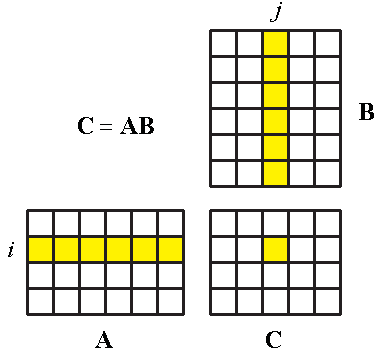
\includegraphics[width=7cm]{./figures/Mat1.pdf}
\caption{矩阵乘法的示意图: $\mat C$ 的 $(i, j)$ 矩阵元等于 $\mat A$ 的第 $i$ 行和 $\mat B$ 的第 $j$ 列逐个元素相乘再相加} \label{Mat_fig1}
\end{figure}

矩阵乘法一般不满足交换律,举一个反例:
\begin{equation}
\pmat{ 1 & 1\\ 0 & 0 }
\pmat{ 1 & 0\\ 1 & 0 } =
\pmat{ 2 & 0\\ 0 & 0 } \ne
\pmat{ 1 & 1\\ 1 & 1 } =
\pmat{ 1 & 0\\ 1 & 0 }
\pmat{ 1 & 1\\ 0 & 0 }
\end{equation}

\subsection{矩阵的乘法分配律}
矩阵的乘法满足分配律
\begin{equation}\label{Mat_eq13}
\mat A (\mat B + \mat C) = \mat A \mat B + \mat A \mat C
\end{equation}
\begin{equation}\label{Mat_eq14}
(\mat A + \mat B) \mat C = \mat A \mat C + \mat B \mat C
\end{equation}
令\autoref{Mat_eq13} 左边等于矩阵 $\mat D$, 则其矩阵元为
\begin{equation}
D_{ij} = \sum_k A_{ik} (B_{kj} + C_{kj})
\end{equation}
拆括号得
\begin{equation}
D_{ij} = \sum_k A_{ik}B_{kj} + \sum_k A_{ik}C_{kj}
\end{equation}
而这恰好是 $\mat A \mat B + \mat A \mat C$ 的矩阵元. 证毕.\autoref{Mat_eq14} 的证明类似.

现在我们可以得出线性变换(\autoref{Mat_eq5})的一个重要性质. 对若干同长度的列矢量 $\vec v_1, \vec v_2, \dots$
\begin{equation}
\mat A \qty(\sum_i c_i \vec v_i) = \sum_i c_i \mat A \vec v_i
\end{equation}
也就是说若干列矢量的线性组合的线性变换等于每个列矢量分别进行线性变换再进行同样的线性组合.

\subsection{矩阵乘法的结合律}
现在来看三个矩阵相乘,令
\begin{equation}
\mat D = \mat A (\mat B\mat C)
\end{equation}
这里的括号是为了强调顺序.即使没有括号,习惯上也是从右向左计算. $\mat D$ 的矩阵元为
\begin{equation}
D_{ij} = \sum_l A_{il} (BC)_{lj} = \sum_l A_{il} \qty(\sum_k B_{lk} C_{kj} )
\end{equation}
拆括号,得
\begin{equation}
D_{ij} = \sum_k\sum_l  ( A_{il} B_{lk} C_{kj} )
\end{equation}
对 $C_{kj}$ 进行合并同类项,得
\begin{equation}
D_{ij} = \sum_k \qty(\sum_l A_{il} B_{lk} ) C_{kj} 
\end{equation}
括号中恰好是 $\mat A$ 乘以 $\mat B$ 所得矩阵的矩阵元 $(AB)_{ik}$ 所以
\begin{equation}
D_{ij} = \sum_k (AB)_{ik} C_{kj}
\end{equation}
即
\begin{equation}
\mat D = (\mat A\mat B)\mat C
\end{equation}
证毕.

\subsection{单位矩阵}
\bb{单位矩阵}就是对角线上的元素全为 1, 非对角线上的元素全为 0 的方阵. 通常记为通常记为$\mat I$. 为了强调矩阵的维数 $N$, 也可记为 $\mat I_N$. 单位矩阵的矩阵元可用克罗内克 $\delta$ 函数(\autoref{OrNrB_eq2}\upref{OrNrB})表示为
\begin{equation}
I_{ij} = \delta_{ij}
\end{equation} 
任何矩阵左乘或右乘单位矩阵, 仍然得到矩阵本身. 单位矩阵的转置仍为单位矩阵.

\subsection{逆矩阵}
% 这里并不详细讲逆矩阵, 了解基本概念即可.
记方阵 $\mat M$ 的\bb{逆矩阵}为 $\mat M^{-1}$, 且满足
\begin{equation}
\mat M^{-1} \mat M = \mat I
\end{equation}
其中 $\mat I$ 是单位矩阵. 也就是说, 任意一个矩阵(或列矢量) $\mat A$ 乘以矩阵 $\mat M$ 再乘以其逆矩阵 $\mat M^{-1}$ 仍然得到 $\mat A$ 本身.

虽然矩阵乘法一般不满足交换律, 但矩阵和对应的逆矩阵满足\footnote{这个定理暂时不证}, 即
\begin{equation}
\mat M\mat M^{-1} = \mat M^{-1} \mat M = \mat I
\end{equation}

逆矩阵 $\mat M^{-1}$ 所代表的线性变换就是 $\mat M$ 代表的线性变换的逆变换, 令 $\vec x$ 和 $\vec y$ 为列矢量, 如果有
\begin{equation}\label{Mat_eq25}
\vec y = \mat M \vec x
\end{equation}
那么我们在等式两边左乘 $\mat M^{-1}$ 再把等式左右互换, 则上式变为
\begin{equation}\label{Mat_eq26}
\vec x = \mat M^{-1} \vec y
\end{equation}

要求逆矩阵, 一种简单直接但低效的方法就是先令 $\vec y = (1, 0, \dots)\Tr$, 代入\autoref{InvMat_eq25} 解线性方程组得 $\vec x$, 将 $\vec x, \vec y$ 代入\autoref{InvMat_eq26} 可知 $\vec x$ 就是 $\mat M$ 的第一列, 再令 $\vec y = (0, 1, 0, \dots)\Tr$, 解线性方程组可得 $\mat M$ 的第二列, 以此类推就可以得到完整的 $\mat M$.
